% $Id: $
\documentclass[a4paper, 10pt]{article}
% reduced margins
\usepackage{fullpage}
\usepackage[authoryear]{natbib}
% spacing
\usepackage{setspace}
% page headings
\usepackage{fancyhdr}
%\usepackage{lscape}

\setlength{\headheight}{15.2pt}
\pagestyle{fancy}
% urls

\usepackage{lscape}
\usepackage{graphicx}
\usepackage{color}
\usepackage{hyperref}
\usepackage{url}
\hypersetup{colorlinks, urlcolor=darkblue}
\usepackage{enumerate}



% figs to be 75% of test width
\setkeys{Gin}{width=0.75\textwidth}

\usepackage[utf8]{inputenc}
\usepackage{graphicx}

\usepackage{lscape}
\usepackage{graphicx}
\usepackage{color}
\usepackage[table]{xcolor}
 
\definecolor{gray90}{gray}{0.95}
\definecolor{gray80}{gray}{0.90}
\definecolor{gray70}{gray}{0.85}
\definecolor{gray60}{gray}{0.80}
\definecolor{gray50}{gray}{0.75}

\usepackage{tikz}
%
\renewcommand{\abstractname}{\large SUMMARY}
%
\newcommand{\Keywords}[1]{\begin{center}\par\noindent{{\em KEYWORDS\/}: #1}\end{center}}
%
\makeatletter
\renewcommand{\subsubsection}{\@startsection{subsubsection}{3}{\z@}%
  {-1.25ex\@plus -1ex \@minus -.2ex}%
  {1.5ex \@plus .2ex}%
  {\normalfont\slshape}}
\renewcommand{\subsection}{\@startsection{subsection}{2}{\z@}%
  {-3.25ex\@plus -1ex \@minus -.2ex}%
  {1.5ex \@plus .2ex}%
  {\normalfont\bfseries\slshape}}
\renewcommand{\section}{\@startsection{section}{1}{\z@}%
  {-5.25ex\@plus -1ex \@minus -.2ex}%
  {1.5ex \@plus .2ex}%
  {\normalfont\bfseries}}
\makeatother
%
\renewcommand\thesection{\arabic{section}}
\renewcommand\thesubsection{\thesection\arabic{subsection}}
\renewcommand\thesubsubsection{\thesubsection\arabic{subsubsection}}
%
\renewcommand{\headrulewidth}{0pt}

\usepackage{listings}

\newenvironment{mylisting}
{\begin{list}{}{\setlength{\leftmargin}{1em}}\item\scriptsize\bfseries}
{\end{list}}

\newenvironment{mytinylisting}
{\begin{list}{}{\setlength{\leftmargin}{1em}}\item\tiny\bfseries}
{\end{list}}

\usepackage{listings}

\definecolor{darkblue}{rgb}{0,0,0.5}
\definecolor{shadecolor}{rgb}{1,1,0.95}
\definecolor{shade}{rgb}{1,1,0.95}


\lstset{ %
language=R,   % the language of the code
basicstyle=\footnotesize, % the size of the fonts that are used for the code
numbers=left,   % where to put the line-numbers
numberstyle=\footnotesize, % the size of the fonts that are used for the line-numbers
stepnumber=100,   % the step between two line-numbers. If it's 1, each line 
    % will be numbered
numbersep=5pt,   % how far the line-numbers are from the code
backgroundcolor=\color{shade}, % choose the background color. You must add \usepackage{color}
showspaces=false,  % show spaces adding particular underscores
showstringspaces=false,  % underline spaces within strings
showtabs=false,   % show tabs within strings adding particular underscores
frame=single,   % adds a frame around the code
tabsize=2,   % sets default tabsize to 2 spaces
captionpos=b,   % sets the caption-position to bottom
breaklines=true,  % sets automatic line breaking
breakatwhitespace=false, % sets if automatic breaks should only happen at whitespace
title=\lstname,   % show the filename of files included with \lstinputlisting;
    % also try caption instead of title
escapeinside={\%*}{*)},  % if you want to add a comment within your code
morekeywords={*,...}  % if you want to add more keywords to the set
}

%
\title{Projections for East Atlantic Mediterranean Bluefin Tuna.}
%
\author{Laurence T. Kell\footnote{{ICCAT Secretariat, C/Coraz\'{o}n de Mar\'{\i}a, 8. 28002 Madrid, Spain; ~Laurie.Kell@iccat.int; ~Phone: +34 914 165 600 ~Fax: +34 914 152 612.}}, 
        Sylvain Bonhommeau\footnote{{IFREMER - UMR EME 212, Av. Jean Monnet, 34200 S\`ete, France;~sylvain.bonhommeau@ifremer.fr; ~Phone: +33 499 57 32 66 ~Fax: +33 499 57 32 95.}},\\
        Jean-Marc Fromentin\footnotemark[2],
        Mauricio Ortiz\footnotemark[1], 
        John Walter\footnote{{ NOAA-Fisheries SEFSC, 75 Virginia Beach Drive, Miami, Florida 33149, USA. john.f.walter@noaa.gov}}}
%
\date{}
%
\begin{document}


\onehalfspacing
\lhead{\normalsize\textsf{SCRS/2012/186}}
\rhead{}

\maketitle
% gets headers on title page ...
\thispagestyle{fancy}
% ... but not on others
\pagestyle{empty}

%
\begin{abstract}

\textit{The management plan for East Atlantic and Mediterranean bluefin tuna is bsed on the Kobe II strategy matrix (K2SM), which indicates the probability 
of $SSB \textgreater B_{MSY}$ and $F \textless F_{MSY}$ for different levels of catch  projections. In this paper we  document the
projections for Eastern Atlantic and Mediterranean bluefin tuna.}

\end{abstract}

\Keywords{stock assessment; bluefin tuna}

 
 
\newpage
\section[Introduction]{Introduction}

The management plan for East Atlantic and Mediterranean bluefin tuna is bsed on the Kobe II strategy matrix (K2SM), which indicates the probability 
of $SSB \textgreater B_{MSY}$ and $F \textless F_{MSY}$ for different levels of catch for a range of projection years.
Resolution [11-14] summarised how the scientific information, modeling approaches and assumptions underpinning management advice should be presented 
in the SCRS annual reports and working group detailed reports. Since the projections were performed after the stock assessment working we do this 
in this document for East Atlantic and Mediterranean bluefin tuna.

\section[Material and Methods]{Material and Methods}

A full description of the stock assessment method, assumptions and data used can be found in the detailed report (SCRS, 2012). 
The longterm management plan is based on the Virtual Population Analysis (VPA) conducted in 2010 (SCRS, 2011). In 2010 four VPA scenarios 
were considered i.e. two levels of catch and two sets of catch per unit effort series. Catches used were either the reported or inflated 
scenario where the catches were raised 
to 50,000 tonnes from 1998 to 2006 and to 61,000 tonnes in 2007. The two sets of CPUE series considered differed by how the juvenile baitboat 
indices were included (i.e. by using either the nominal or standardised series). The reason for this was because management measures had 
affected these series making standardisation problematic. However as these were the only index for juvenile bluefin in the East Atlantic 
there inclusion was considered important.

In 2010 twenty four projection scenarios were run using Pro-2box to construct the K2SM. As  well as the four VPA runs, there were three 
recruitment scenarios and two assummed future selection patterns. The three recruitment scenarios acknowledged that there was insufficient 
scientific information to determine precisely the productivity of the stock (i.e. the steepness of the stock-recruitment relationship) the 
projections had been conducted with three recruitment levels while taking into account for year-to-year variations. These levels correspond 
to the ‘low’ and ‘high’ scenarios as defined in the 2008 assessment plus a ‘Medium’ scenario that corresponds to the geometric mean of the 
recruitment over the 1950-2006 years. The two selection patterns corresponded to different assumptions about the effectiveness of management 
regulations in reducing catches of juveniles.

In 2012 only six projection scenarios (two catch and recruitement levels) were used to create the K2SM. A single index of juveniles had been 
constructed based on the Bay of Biscay baitboat fleet (SCRS/2012/xxx) and so only two VPA scenarios (i.e. reported and inflated catches) were 
considered when running the projections. The group also considered that it was 
now possible to estimate the changes in selection pattern and so only one selectivity scenario was used to create the K2SM. Three
recruitment scenarios (low, medium and high) were considered as before. For comparison with the 2010 projections six scenarios were
run with the selection pattern from 2010 where it had been assummed measures had been implemented perfectly. However, these
were not used to construct the kobe matrix.

Projections were carried out using VPA Run 2, with both the reported and inflated catches (but no inflation of reported catch since 2008). 
When projecting it is necessary to specify, biological parameters, selection pattern (including any modifications due to technical measures 
that may be implemented), recruitment. Numbers-at-age are poorly estimated for the recent year classes by VPA. Therefore 
the first three ages in the initial population vector (i.e. for 2009, 2010, and 2011) were replaced with a random value 
from the stochastic recruitment specifications. These values were then projected forward in time accounting for the observed catches and the 
assumed natural mortality at age. This results in changes to both the number at age in 2012 (i.e. the first projection year) and the fishing 
mortality and selectivity-at-age for the three year-classes replaced. The current estimated selectivity pattern was 
calculated as the geometric mean of the most recent three years i.e.  2009,2010 and 2011 in 2012, 
similar to the one used in the 2010 projections for calculating benchmarks.
The plusgroup in the projections was age 10, to ensure consistency with the historic assessment. Weights-at-age in the 
projections were computed from the growth curve, this included using the average age of the plus-group to calculate the 
mean weight of individuals in the plusgroup.

\section[Results]{Results}

The selectivity pattern used in the projections are summarised in (figure~\ref{fig:1}); these show the medians (lines) 
and $\pm$ 1 sd (bars). These correspond to the reported and inflated catches and, for comparison purposes 
the \emph{perfect implementation} selectivity pattern used in the 2010 projections and the current selectivity pattern. The current 
selectivity pattern was calculated independently for each bootstrap. 
For the calculation of benchmarks and projections based on the 2010 selectivity pattern, the 2012 selectivity
pattern was modified by applying a vector (i.e. the ratio of the selectivities estimated in 2010 and 2012 based on their 
geometric means) to obtain the same selectivities as used in 2010.


Figure~\ref{fig:2} shows the Kobe plot for stock relative to $B_{MSY}$ and harvest
rate relative to $F_{MSY}$ as estimated in 2012, for the two selectivity patterns (rows), catch scenarios 
(columns) and recruitment scenarios (colors). The lines show the medians from 2008 to 2011 and the 
points the bootstraps in 2011. The green quadrant corresponds to the stock not being overfished and no overfishing occurring and 
the red quadrant to the stock being overfished and overfishing occurring.

The differences in the 2011 estimates of being in the kobe quadrants are summarised as a pie chart in (figure~\ref{fig:3}). 
These show the proportion of the VPA estimates in 
terminal year (2011) that are within the green quadrant of the Kobe plot chart (not overfished, no overfishing), 
the yellow quadrant (overfished or overfishing), and the red quadrant (overfished and overfishing). 
Split by catch scenario (reported and inflated) and benchmark (2010 and 2012).

The differences due to assuming benchmarks based upon 2010 or 2012 selectivities as summarised in figure~\ref{fig:4}.

The kobe matrices are summarised graphically in figure~\ref{fig:5} and as tables in
tables 1, 2 and 3. These indicate the probabilities of  $F \textless F_{MSY}$, $B$ \textgreater $B_{MSY}$ and $B \textgreater B_{MSY}$ and 
$F \textless F_{MSY}$ for quotas from 0 to 30000t for 2013 through 2022.
Shading corresponds to the probabilities of being in he ranges of 50-59 \%, 60- 69 \%, 70-79 \%, 80-89 \% and greater or equal to 90 \%.

 


\newpage
\section[Figures]{Figures}

\begin{figure}[!ht]\begin{center}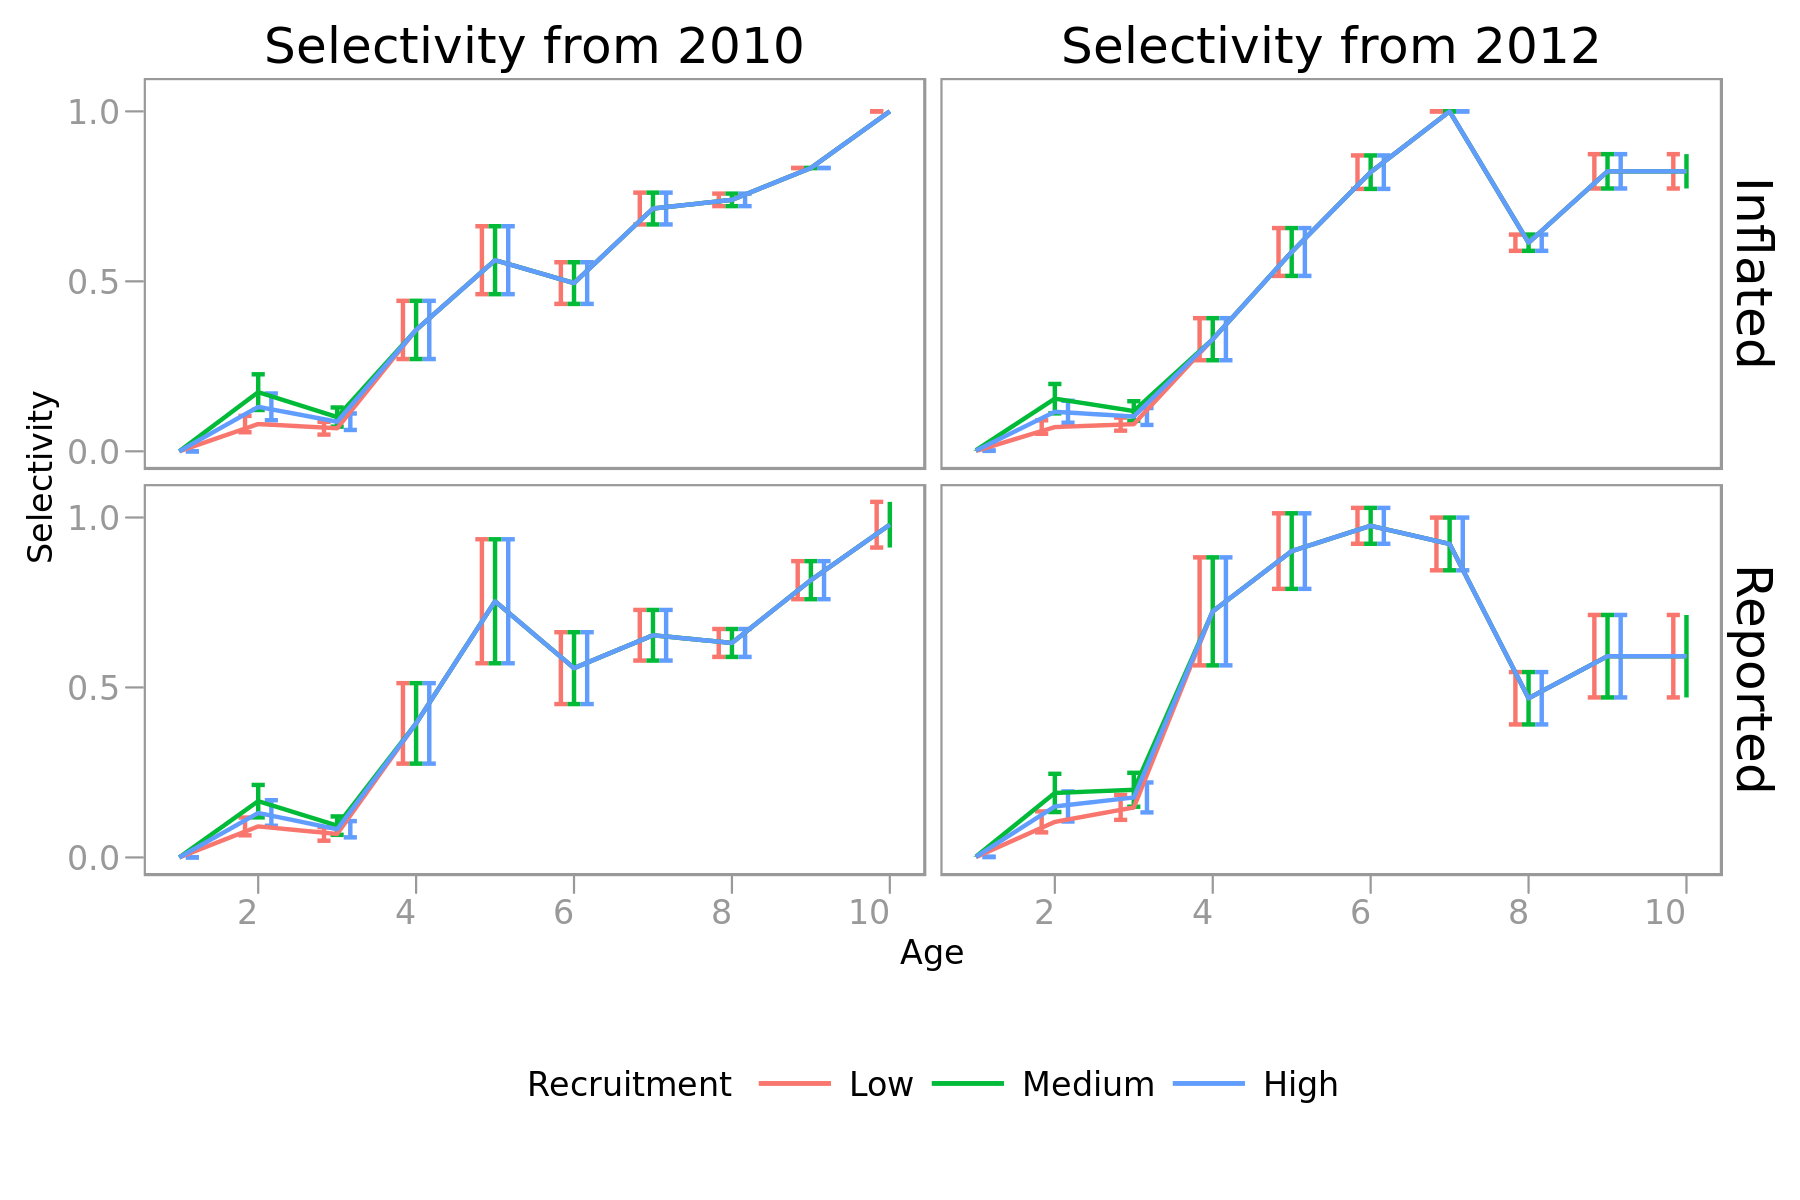
\includegraphics[width=6in]{7_1_1.png}\end{center}
\caption{Vectors of selectivity-at-age used in the projections from the 2010 and 2012 assessments. 
The 2012 selectivities were obtained as the geometric mean of the fishing mortality at age for the last three years of each assessment, 
after applying the 3-year recruitment patch. The 2010 selectivity pattern was that used in the projections made in 2010 assessment}
\label{fig:1}\end{figure}

\begin{figure}[!ht]\begin{center}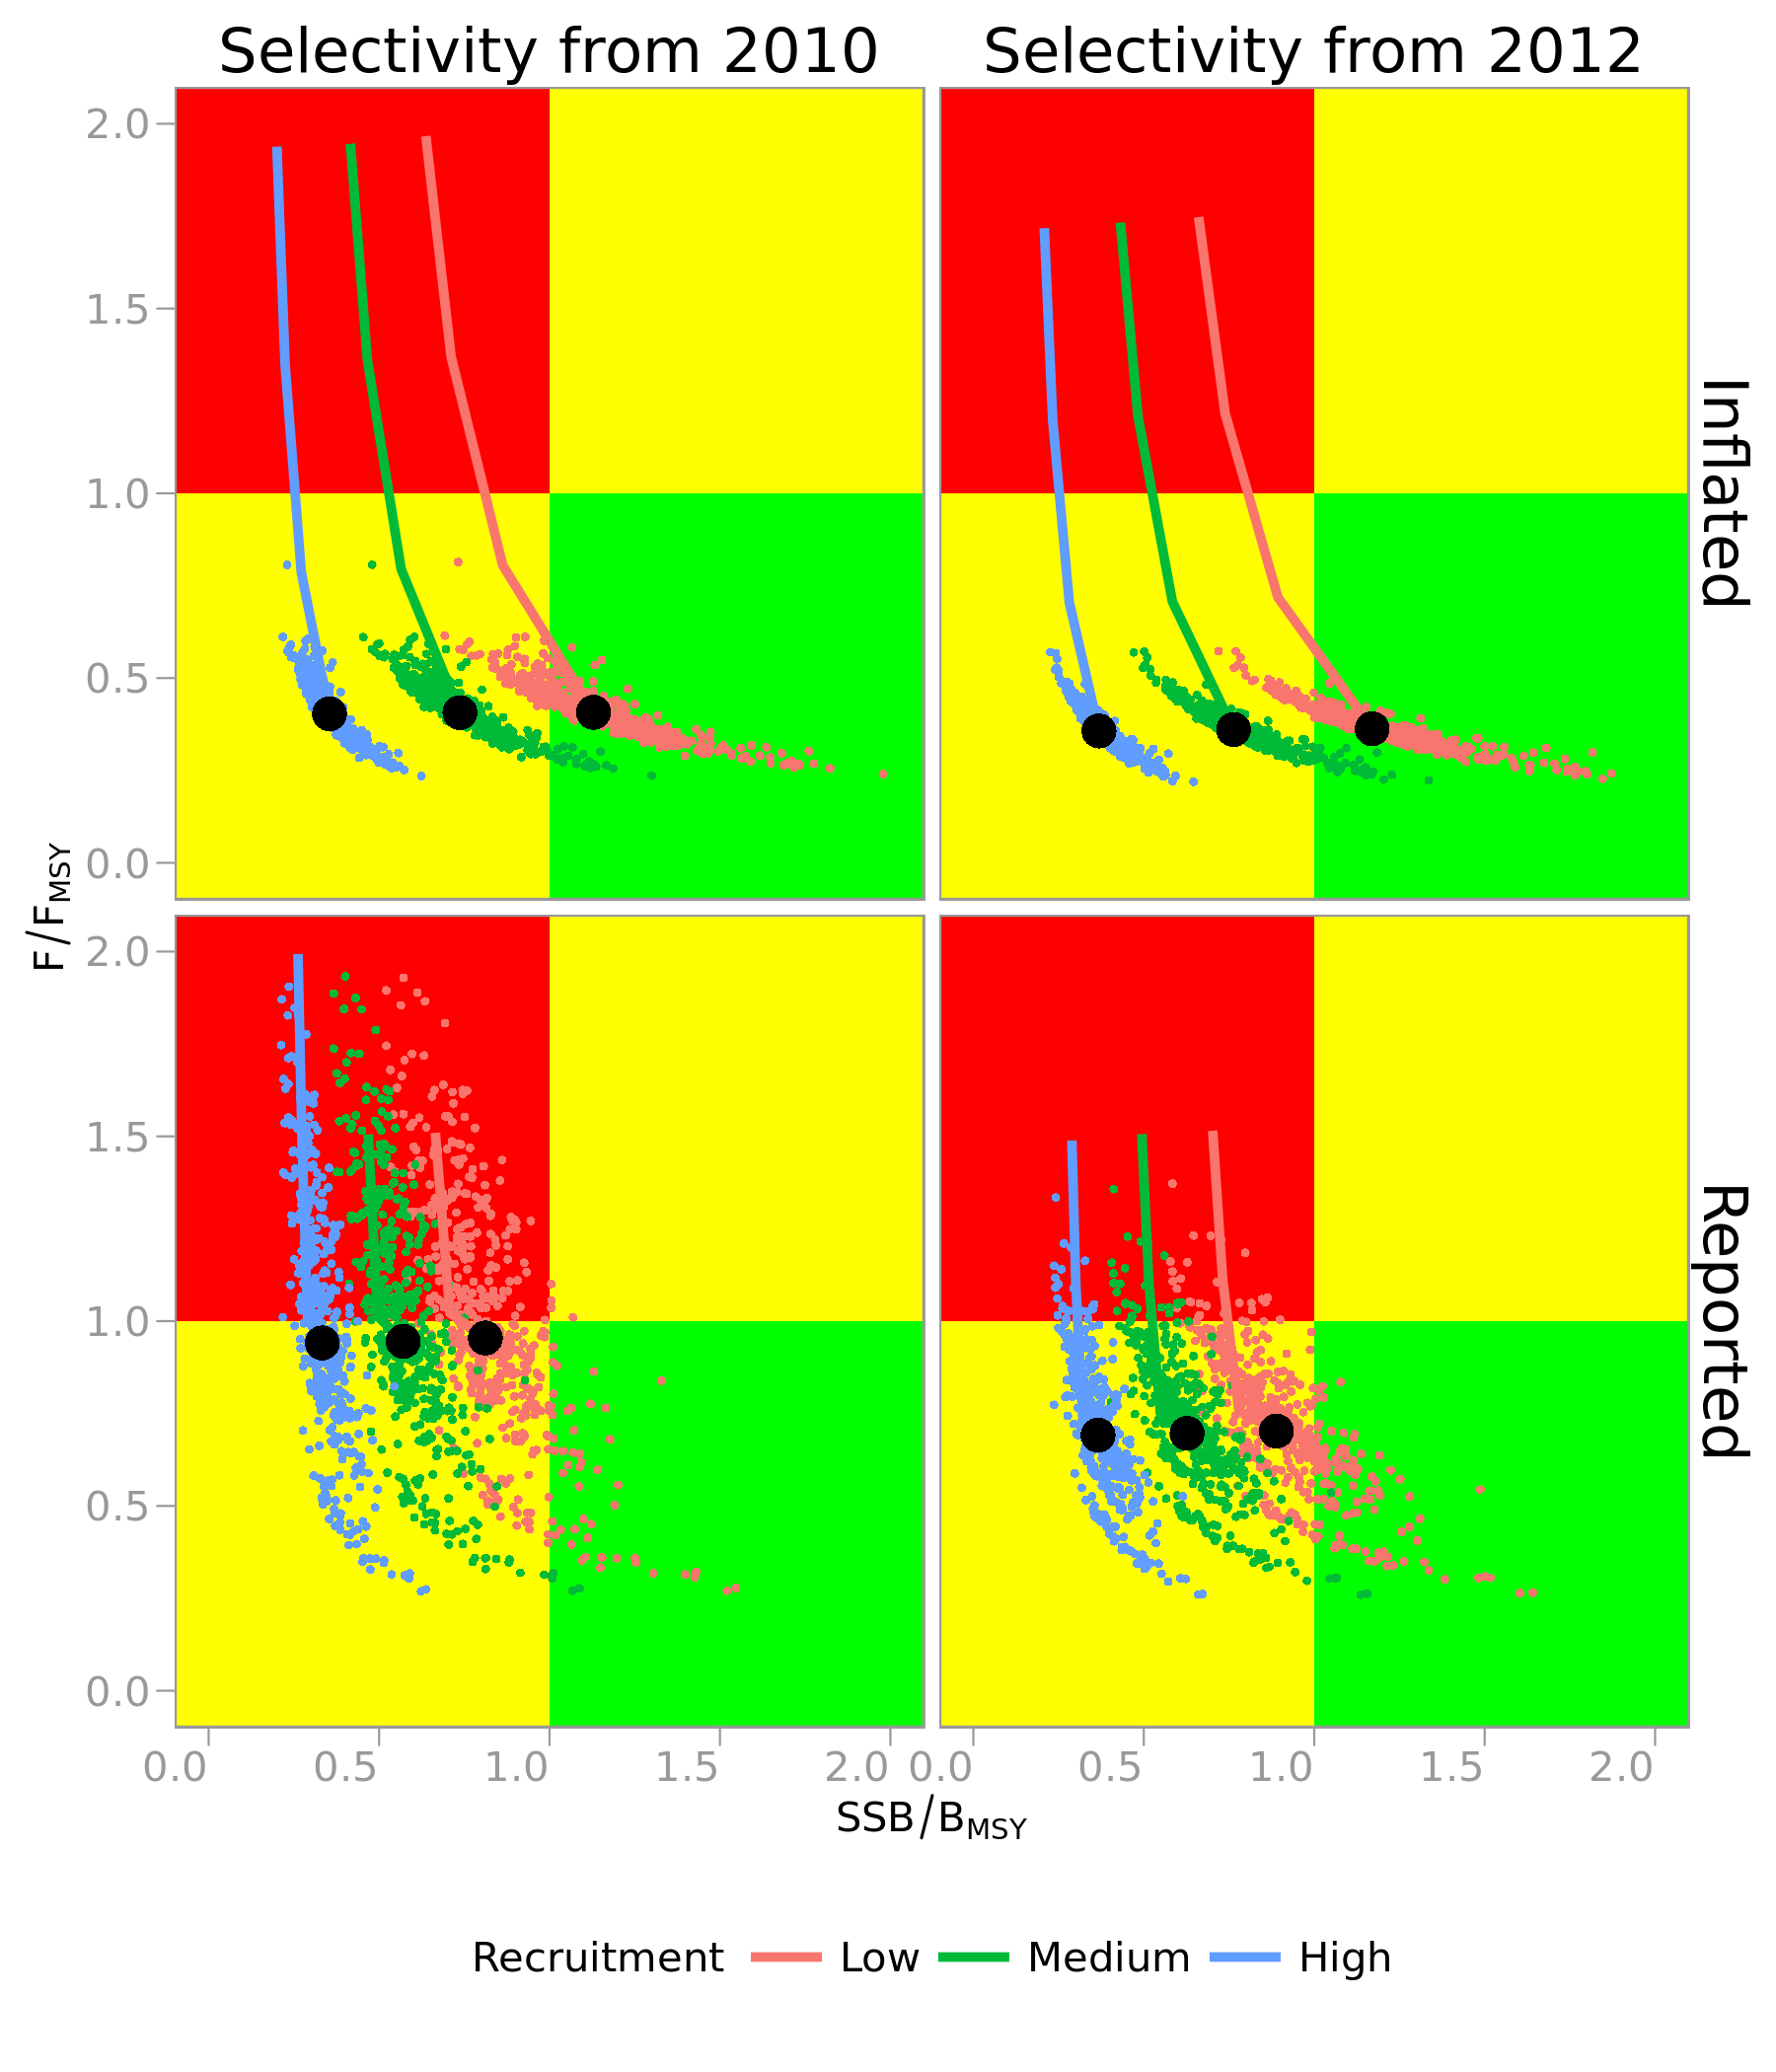
\includegraphics[width=6in]{6_1_9.png}\end{center}
\caption{Figure 6.1.9. Kobe plot for 2011 stock status, individual realisations starting in 
2008 with median for the two selectivity patterns (rows) and the catch scenarios 
(reported or inflated; column) and for the three recruitment scenarios (colors).}
\label{fig:2}\end{figure}

\begin{figure}[!ht]\begin{center}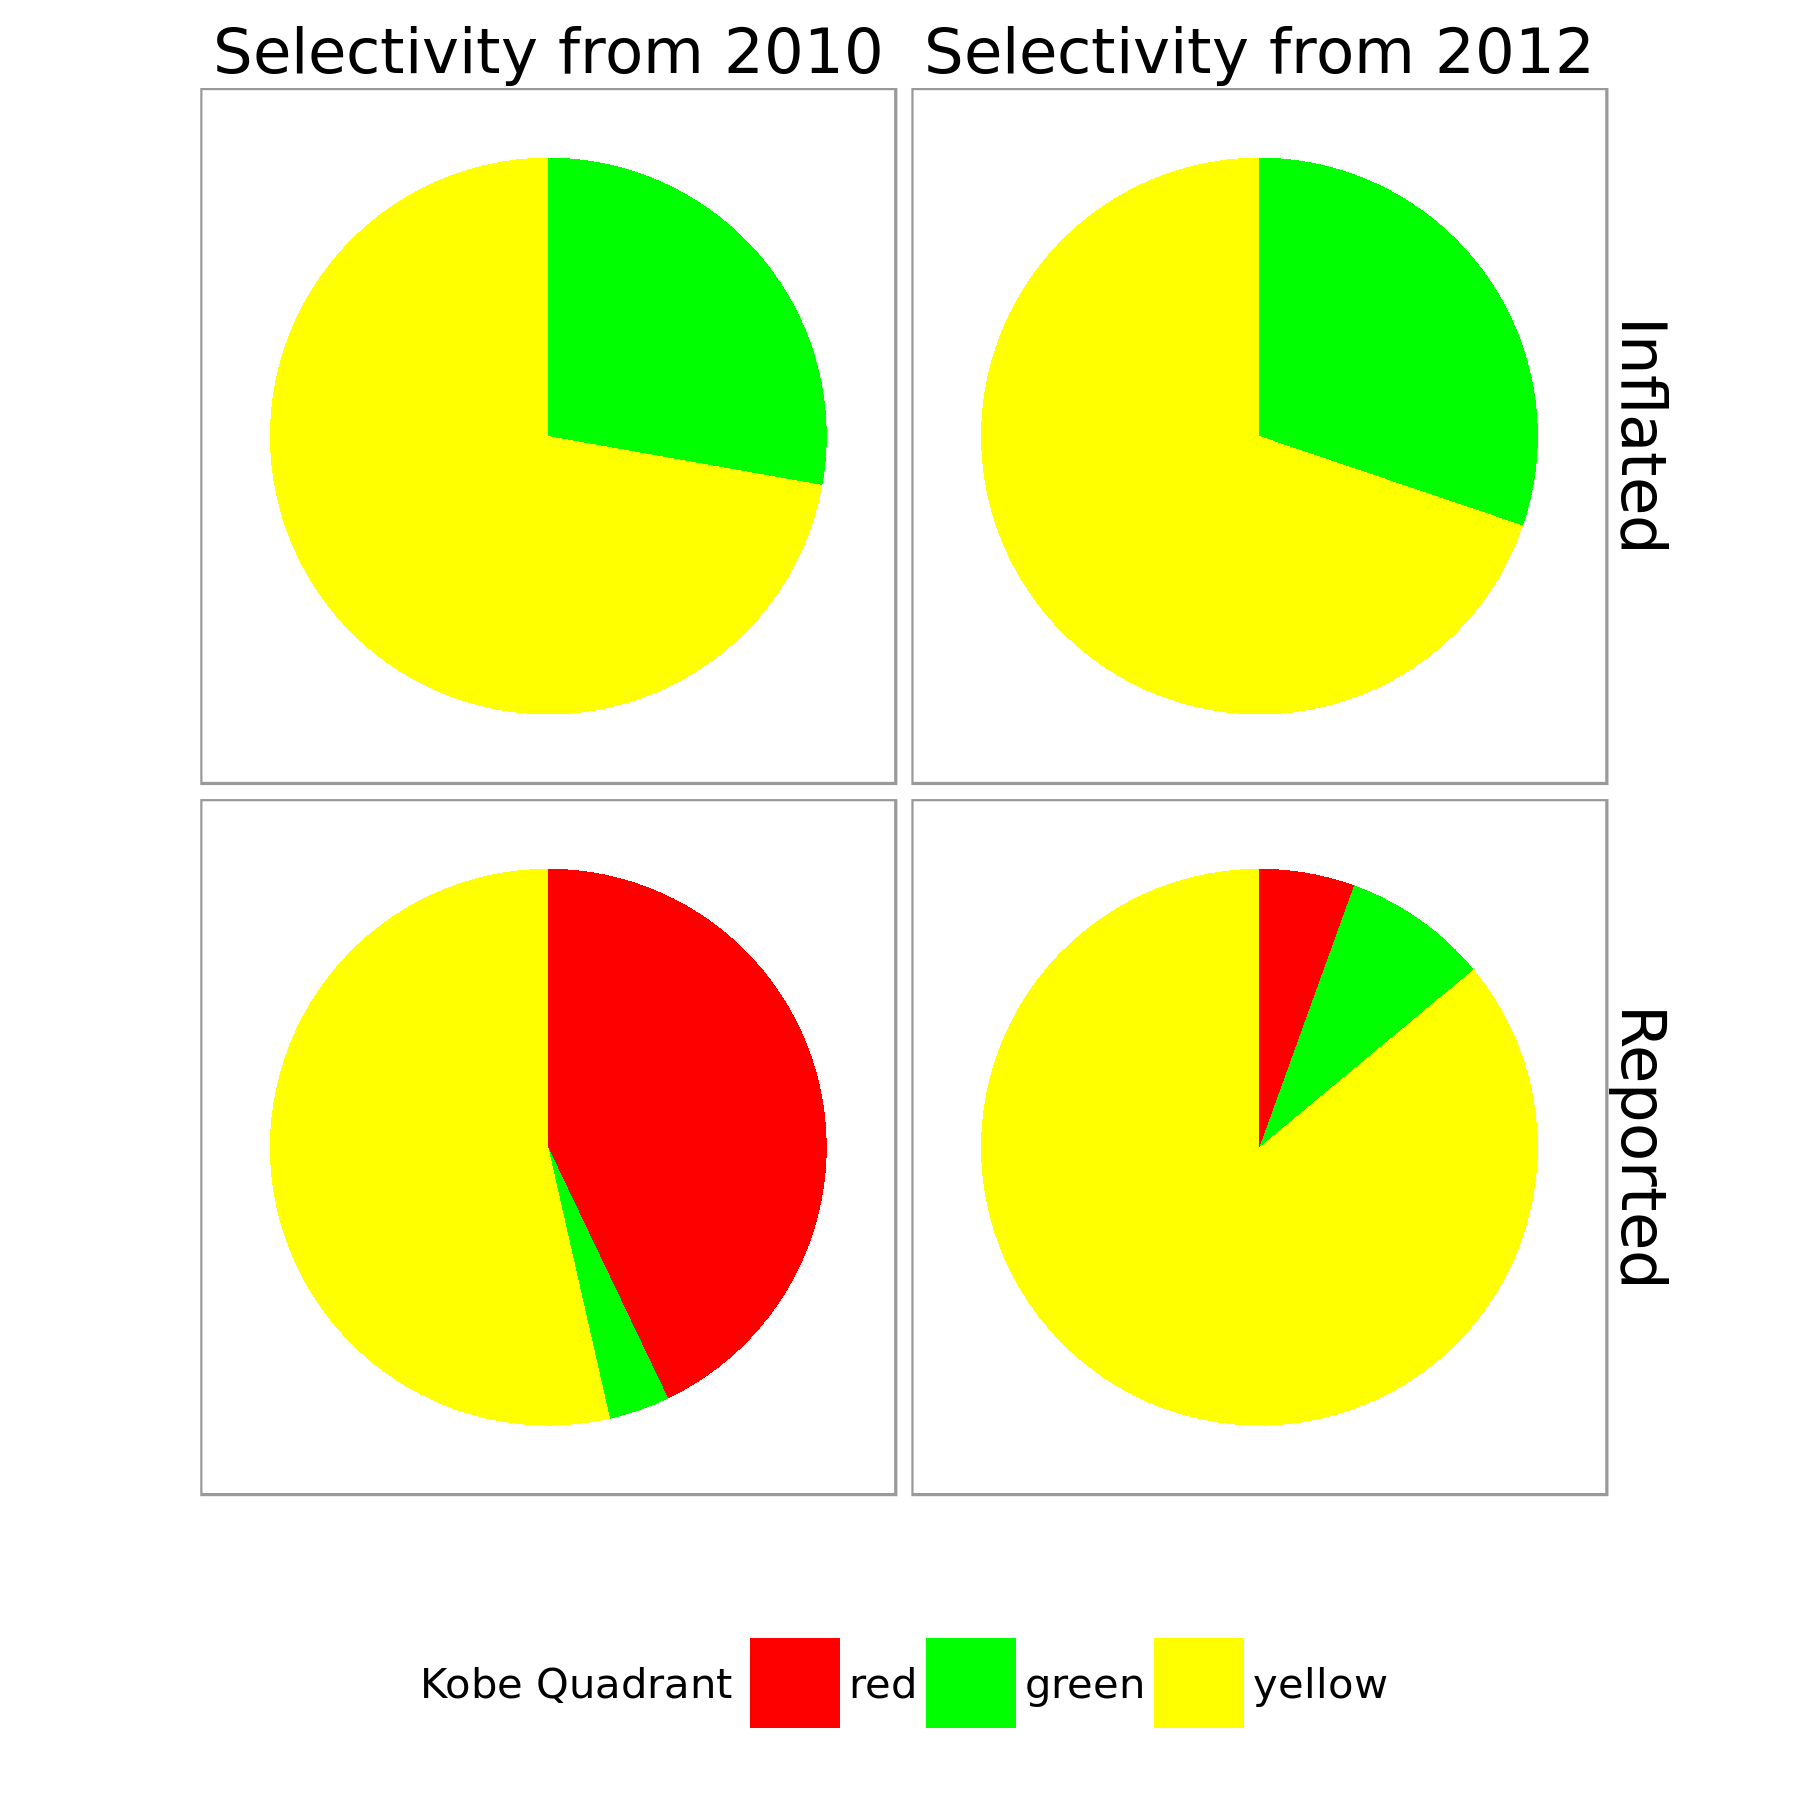
\includegraphics[width=6in]{7_1_2.png}\end{center}
\caption{Figure 7.1.2 Pie chart showing the proportion of the VPA continuity run results for the 
terminal year (2011) that are within the green quadrant of the Kobe plot chart (not overfished, no overfishing), 
the yellow quadrant (overfished or overfishing), and the red quadrant (overfished and overfishing). 
Split by catch scenario (reported and inflated) and benchmark (2010 and 2012).}
\label{fig:3}\end{figure}

\begin{figure}[!ht]\begin{center}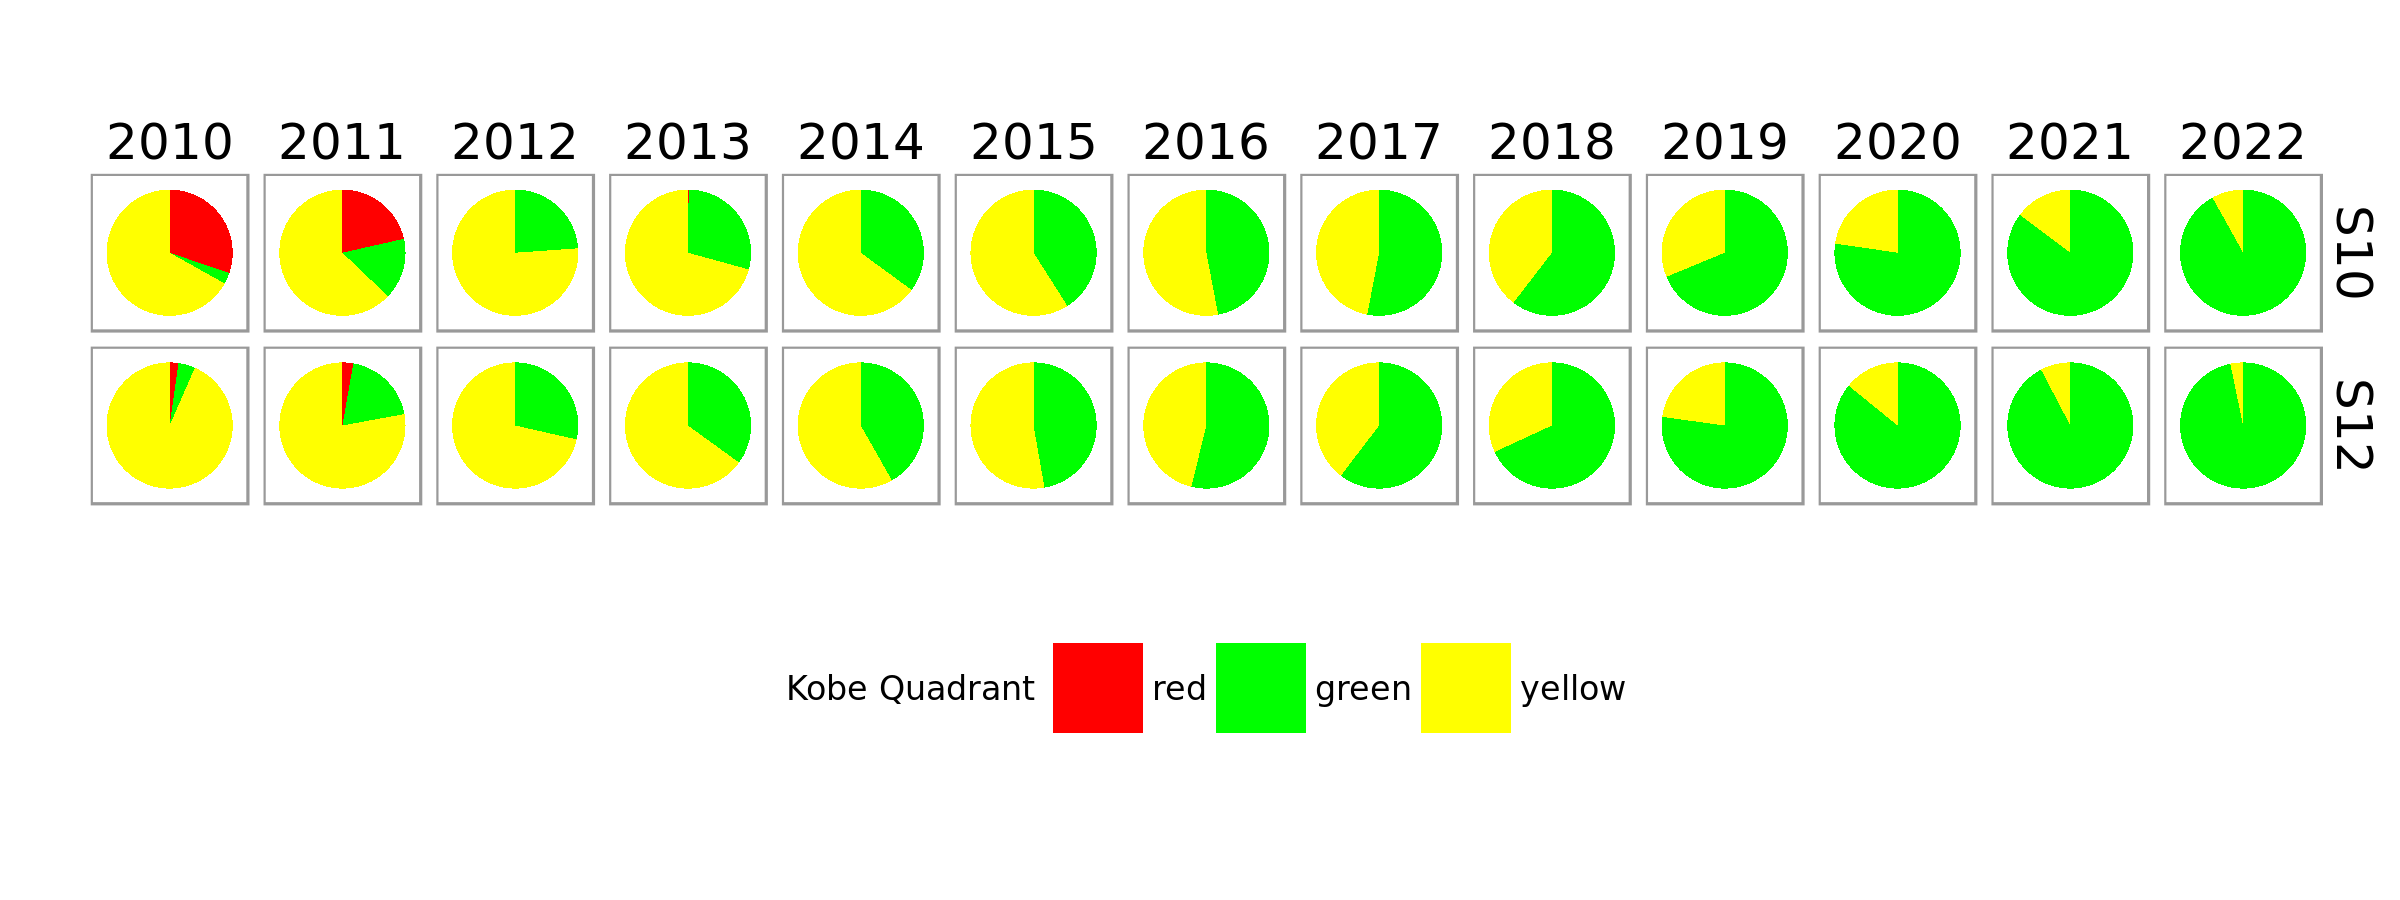
\includegraphics[width=6in]{7_1_3.png}\end{center}
\caption{Figure 7.1.3: Pie chart showing the proportion of the VPA continuity run results for the terminal year (2011) 
that are within the green quadrant of the Kobe plot chart (not overfished, no overfishing), the yellow quadrant 
(overfished or overfishing), and the red quadrant (overfished and overfishing). Split by benchmark (i.e. as estimated in 2010 and 2012)
and integrating over the 3 recruitment (low, medium and high) and two catch scenarios (reported and inflated).}
\label{fig:4}\end{figure}

\begin{figure}[!ht]\begin{center}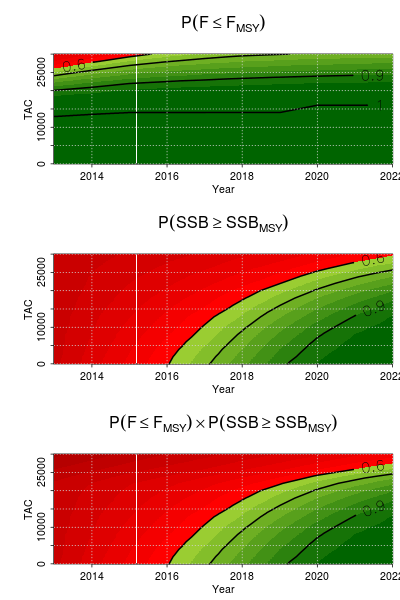
\includegraphics[width=6in]{k2sm.png}\end{center}
\caption{Kobe II strategy matrices, indicating the probabilities of  $F \textless F_{MSY}$, $B$ \textgreater $B_{MSY}$ and $B \textgreater B_{MSY}$ and 
$F \textless F_{MSY}$ for quotas from 0 to 30000t for 2013 through 2022.}
\label{fig:5}\end{figure}

\clearpage
\newpage

% latex.default(kobeShade(k2smTab[[1]], pct = ""), file = paste(dirTex,      "k2smF.tex", sep = "/"), rowlabel = "TAC", rowname = dimnames(k2smTab[[1]])$TAC,      caption = "Kobe II Strategy Matrix, $P(F\\leq F_{MSY})$.") 
%
\begin{table}[!tbp]
\caption{Kobe II Strategy Matrix, $P(F\leq F_{MSY})$.\label{kobeShade}} 
\begin{center}
\begin{tabular}{lllllllllll}
\hline\hline
\multicolumn{1}{l}{TAC}&\multicolumn{1}{c}{2013}&\multicolumn{1}{c}{2014}&\multicolumn{1}{c}{2015}&\multicolumn{1}{c}{2016}&\multicolumn{1}{c}{2017}&\multicolumn{1}{c}{2018}&\multicolumn{1}{c}{2019}&\multicolumn{1}{c}{2020}&\multicolumn{1}{c}{2021}&\multicolumn{1}{c}{2022}\tabularnewline
\hline
0&\cellcolor{gray50} 100&\cellcolor{gray50} 100&\cellcolor{gray50} 100&\cellcolor{gray50} 100&\cellcolor{gray50} 100&\cellcolor{gray50} 100&\cellcolor{gray50} 100&\cellcolor{gray50} 100&\cellcolor{gray50} 100&\cellcolor{gray50} 100\tabularnewline
2000&\cellcolor{gray50} 100&\cellcolor{gray50} 100&\cellcolor{gray50} 100&\cellcolor{gray50} 100&\cellcolor{gray50} 100&\cellcolor{gray50} 100&\cellcolor{gray50} 100&\cellcolor{gray50} 100&\cellcolor{gray50} 100&\cellcolor{gray50} 100\tabularnewline
4000&\cellcolor{gray50} 100&\cellcolor{gray50} 100&\cellcolor{gray50} 100&\cellcolor{gray50} 100&\cellcolor{gray50} 100&\cellcolor{gray50} 100&\cellcolor{gray50} 100&\cellcolor{gray50} 100&\cellcolor{gray50} 100&\cellcolor{gray50} 100\tabularnewline
6000&\cellcolor{gray50} 100&\cellcolor{gray50} 100&\cellcolor{gray50} 100&\cellcolor{gray50} 100&\cellcolor{gray50} 100&\cellcolor{gray50} 100&\cellcolor{gray50} 100&\cellcolor{gray50} 100&\cellcolor{gray50} 100&\cellcolor{gray50} 100\tabularnewline
8000&\cellcolor{gray50} 100&\cellcolor{gray50} 100&\cellcolor{gray50} 100&\cellcolor{gray50} 100&\cellcolor{gray50} 100&\cellcolor{gray50} 100&\cellcolor{gray50} 100&\cellcolor{gray50} 100&\cellcolor{gray50} 100&\cellcolor{gray50} 100\tabularnewline
10000&\cellcolor{gray50} 100&\cellcolor{gray50} 100&\cellcolor{gray50} 100&\cellcolor{gray50} 100&\cellcolor{gray50} 100&\cellcolor{gray50} 100&\cellcolor{gray50} 100&\cellcolor{gray50} 100&\cellcolor{gray50} 100&\cellcolor{gray50} 100\tabularnewline
12000&\cellcolor{gray50} 100&\cellcolor{gray50} 100&\cellcolor{gray50} 100&\cellcolor{gray50} 100&\cellcolor{gray50} 100&\cellcolor{gray50} 100&\cellcolor{gray50} 100&\cellcolor{gray50} 100&\cellcolor{gray50} 100&\cellcolor{gray50} 100\tabularnewline
12900&\cellcolor{gray50} 100&\cellcolor{gray50} 100&\cellcolor{gray50} 100&\cellcolor{gray50} 100&\cellcolor{gray50} 100&\cellcolor{gray50} 100&\cellcolor{gray50} 100&\cellcolor{gray50} 100&\cellcolor{gray50} 100&\cellcolor{gray50} 100\tabularnewline
13500&\cellcolor{gray50} 100&\cellcolor{gray50} 100&\cellcolor{gray50} 100&\cellcolor{gray50} 100&\cellcolor{gray50} 100&\cellcolor{gray50} 100&\cellcolor{gray50} 100&\cellcolor{gray50} 100&\cellcolor{gray50} 100&\cellcolor{gray50} 100\tabularnewline
14000&\cellcolor{gray50} 100&\cellcolor{gray50} 100&\cellcolor{gray50} 100&\cellcolor{gray50} 100&\cellcolor{gray50} 100&\cellcolor{gray50} 100&\cellcolor{gray50} 100&\cellcolor{gray50} 100&\cellcolor{gray50} 100&\cellcolor{gray50} 100\tabularnewline
16000&\cellcolor{gray50} 99&\cellcolor{gray50} 100&\cellcolor{gray50} 100&\cellcolor{gray50} 100&\cellcolor{gray50} 100&\cellcolor{gray50} 100&\cellcolor{gray50} 100&\cellcolor{gray50} 100&\cellcolor{gray50} 100&\cellcolor{gray50} 100\tabularnewline
18000&\cellcolor{gray50} 97&\cellcolor{gray50} 98&\cellcolor{gray50} 99&\cellcolor{gray50} 99&\cellcolor{gray50} 100&\cellcolor{gray50} 100&\cellcolor{gray50} 100&\cellcolor{gray50} 100&\cellcolor{gray50} 100&\cellcolor{gray50} 100\tabularnewline
20000&\cellcolor{gray50} 93&\cellcolor{gray50} 95&\cellcolor{gray50} 97&\cellcolor{gray50} 97&\cellcolor{gray50} 98&\cellcolor{gray50} 98&\cellcolor{gray50} 98&\cellcolor{gray50} 99&\cellcolor{gray50} 99&\cellcolor{gray50} 99\tabularnewline
22000&\cellcolor{gray60} 86&\cellcolor{gray60} 89&\cellcolor{gray50} 92&\cellcolor{gray50} 93&\cellcolor{gray50} 94&\cellcolor{gray50} 94&\cellcolor{gray50} 94&\cellcolor{gray50} 95&\cellcolor{gray50} 95&\cellcolor{gray50} 95\tabularnewline
24000&\cellcolor{gray70} 77&\cellcolor{gray60} 81&\cellcolor{gray60} 85&\cellcolor{gray60} 86&\cellcolor{gray60} 88&\cellcolor{gray60} 89&\cellcolor{gray60} 89&\cellcolor{gray60} 90&\cellcolor{gray60} 90&\cellcolor{gray60} 90\tabularnewline
26000&\cellcolor{gray80} 68&\cellcolor{gray70} 73&\cellcolor{gray70} 78&\cellcolor{gray70} 80&\cellcolor{gray60} 81&\cellcolor{gray60} 82&\cellcolor{gray60} 83&\cellcolor{gray60} 83&\cellcolor{gray60} 84&\cellcolor{gray60} 84\tabularnewline
28000&\cellcolor{gray90} 59&\cellcolor{gray80} 65&\cellcolor{gray80} 70&\cellcolor{gray70} 73&\cellcolor{gray70} 74&\cellcolor{gray70} 76&\cellcolor{gray70} 76&\cellcolor{gray70} 77&\cellcolor{gray70} 77&\cellcolor{gray70} 78\tabularnewline
30000&\cellcolor{gray90} 51&\cellcolor{gray90} 57&\cellcolor{gray80} 62&\cellcolor{gray80} 66&\cellcolor{gray80} 68&\cellcolor{gray80} 70&\cellcolor{gray70} 70&\cellcolor{gray70} 71&\cellcolor{gray70} 71&\cellcolor{gray70} 71\tabularnewline
\hline
\end{tabular}
\end{center}
\end{table}


% latex.default(kobeShade(k2smTab[[2]], pct = ""), file = paste(dirTex,      "k2smB.tex", sep = "/"), rowlabel = "TAC", rowname = dimnames(k2smTab[[1]])$TAC,      caption = "Kobe II Strategy Matrix, $P(SSB\\geq B_{MSY})$).") 
%
\begin{table}[!tbp]
\caption{Kobe II Strategy Matrix, $P(SSB\geq B_{MSY})$).\label{kobeShade}} 
\begin{center}
\begin{tabular}{lllllllllll}
\hline\hline
\multicolumn{1}{l}{TAC}&\multicolumn{1}{c}{2013}&\multicolumn{1}{c}{2014}&\multicolumn{1}{c}{2015}&\multicolumn{1}{c}{2016}&\multicolumn{1}{c}{2017}&\multicolumn{1}{c}{2018}&\multicolumn{1}{c}{2019}&\multicolumn{1}{c}{2020}&\multicolumn{1}{c}{2021}&\multicolumn{1}{c}{2022}\tabularnewline
\hline
0& 36& 46&\cellcolor{gray90} 54&\cellcolor{gray80} 63&\cellcolor{gray70} 72&\cellcolor{gray60} 82&\cellcolor{gray50} 92&\cellcolor{gray50} 97&\cellcolor{gray50} 100&\cellcolor{gray50} 100\tabularnewline
2000& 36& 45&\cellcolor{gray90} 54&\cellcolor{gray80} 62&\cellcolor{gray70} 70&\cellcolor{gray60} 81&\cellcolor{gray50} 90&\cellcolor{gray50} 97&\cellcolor{gray50} 99&\cellcolor{gray50} 100\tabularnewline
4000& 36& 45&\cellcolor{gray90} 53&\cellcolor{gray80} 61&\cellcolor{gray80} 69&\cellcolor{gray70} 79&\cellcolor{gray60} 89&\cellcolor{gray50} 96&\cellcolor{gray50} 99&\cellcolor{gray50} 100\tabularnewline
6000& 36& 44&\cellcolor{gray90} 52&\cellcolor{gray90} 59&\cellcolor{gray80} 67&\cellcolor{gray70} 77&\cellcolor{gray60} 87&\cellcolor{gray50} 94&\cellcolor{gray50} 98&\cellcolor{gray50} 100\tabularnewline
8000& 36& 43&\cellcolor{gray90} 51&\cellcolor{gray90} 58&\cellcolor{gray80} 66&\cellcolor{gray70} 75&\cellcolor{gray60} 85&\cellcolor{gray50} 92&\cellcolor{gray50} 97&\cellcolor{gray50} 99\tabularnewline
10000& 35& 43& 50&\cellcolor{gray90} 56&\cellcolor{gray80} 64&\cellcolor{gray70} 73&\cellcolor{gray60} 83&\cellcolor{gray50} 91&\cellcolor{gray50} 96&\cellcolor{gray50} 99\tabularnewline
12000& 35& 42& 48&\cellcolor{gray90} 55&\cellcolor{gray80} 63&\cellcolor{gray70} 70&\cellcolor{gray70} 80&\cellcolor{gray60} 88&\cellcolor{gray50} 95&\cellcolor{gray50} 98\tabularnewline
12900& 35& 42& 48&\cellcolor{gray90} 55&\cellcolor{gray80} 62&\cellcolor{gray80} 69&\cellcolor{gray70} 79&\cellcolor{gray60} 87&\cellcolor{gray50} 93&\cellcolor{gray50} 98\tabularnewline
13500& 35& 42& 48&\cellcolor{gray90} 54&\cellcolor{gray80} 61&\cellcolor{gray80} 69&\cellcolor{gray70} 78&\cellcolor{gray60} 87&\cellcolor{gray50} 93&\cellcolor{gray50} 97\tabularnewline
14000& 35& 42& 47&\cellcolor{gray90} 54&\cellcolor{gray80} 60&\cellcolor{gray80} 68&\cellcolor{gray70} 77&\cellcolor{gray60} 86&\cellcolor{gray50} 92&\cellcolor{gray50} 97\tabularnewline
16000& 35& 41& 46&\cellcolor{gray90} 52&\cellcolor{gray90} 58&\cellcolor{gray80} 66&\cellcolor{gray70} 74&\cellcolor{gray60} 83&\cellcolor{gray60} 90&\cellcolor{gray50} 94\tabularnewline
18000& 34& 40& 45&\cellcolor{gray90} 51&\cellcolor{gray90} 56&\cellcolor{gray80} 63&\cellcolor{gray70} 71&\cellcolor{gray70} 79&\cellcolor{gray60} 86&\cellcolor{gray50} 92\tabularnewline
20000& 34& 39& 44& 49&\cellcolor{gray90} 54&\cellcolor{gray80} 60&\cellcolor{gray80} 68&\cellcolor{gray70} 75&\cellcolor{gray60} 83&\cellcolor{gray60} 88\tabularnewline
22000& 34& 39& 43& 47&\cellcolor{gray90} 52&\cellcolor{gray90} 57&\cellcolor{gray80} 63&\cellcolor{gray70} 71&\cellcolor{gray70} 77&\cellcolor{gray60} 83\tabularnewline
24000& 34& 38& 42& 46& 50&\cellcolor{gray90} 55&\cellcolor{gray90} 60&\cellcolor{gray80} 67&\cellcolor{gray70} 73&\cellcolor{gray70} 78\tabularnewline
26000& 34& 37& 41& 44& 48&\cellcolor{gray90} 52&\cellcolor{gray90} 57&\cellcolor{gray80} 62&\cellcolor{gray80} 67&\cellcolor{gray70} 73\tabularnewline
28000& 33& 36& 40& 43& 45& 49&\cellcolor{gray90} 53&\cellcolor{gray90} 58&\cellcolor{gray80} 63&\cellcolor{gray80} 66\tabularnewline
30000& 33& 36& 38& 41& 43& 46& 50&\cellcolor{gray90} 54&\cellcolor{gray90} 58&\cellcolor{gray80} 62\tabularnewline
\hline
\end{tabular}
\end{center}
\end{table}

% latex.default(kobeShade(k2smTab[[3]], pct = ""), file = paste(dirTex,      "k2sm.tex", sep = "/"), rowlabel = "TAC", rowname = dimnames(k2smTab[[1]])$TAC,      caption = "Kobe II Strategy Matrix, $P(F\\leq F_{MSY})$ and $P(SSB\\geq B_{MSY})$.") 
%
\begin{table}[!tbp]
\caption{Kobe II Strategy Matrix, $P(F\leq F_{MSY})$ and $P(SSB\geq B_{MSY})$.\label{kobeShade}} 
\begin{center}
\begin{tabular}{lllllllllll}
\hline\hline
\multicolumn{1}{l}{TAC}&\multicolumn{1}{c}{2013}&\multicolumn{1}{c}{2014}&\multicolumn{1}{c}{2015}&\multicolumn{1}{c}{2016}&\multicolumn{1}{c}{2017}&\multicolumn{1}{c}{2018}&\multicolumn{1}{c}{2019}&\multicolumn{1}{c}{2020}&\multicolumn{1}{c}{2021}&\multicolumn{1}{c}{2022}\tabularnewline
\hline
0& 36& 46&\cellcolor{gray90} 54&\cellcolor{gray80} 63&\cellcolor{gray70} 72&\cellcolor{gray60} 82&\cellcolor{gray50} 92&\cellcolor{gray50} 97&\cellcolor{gray50} 100&\cellcolor{gray50} 100\tabularnewline
2000& 36& 45&\cellcolor{gray90} 54&\cellcolor{gray80} 62&\cellcolor{gray70} 70&\cellcolor{gray60} 81&\cellcolor{gray50} 90&\cellcolor{gray50} 97&\cellcolor{gray50} 99&\cellcolor{gray50} 100\tabularnewline
4000& 36& 45&\cellcolor{gray90} 53&\cellcolor{gray80} 61&\cellcolor{gray80} 69&\cellcolor{gray70} 79&\cellcolor{gray60} 89&\cellcolor{gray50} 96&\cellcolor{gray50} 99&\cellcolor{gray50} 100\tabularnewline
6000& 36& 44&\cellcolor{gray90} 52&\cellcolor{gray90} 59&\cellcolor{gray80} 67&\cellcolor{gray70} 77&\cellcolor{gray60} 87&\cellcolor{gray50} 94&\cellcolor{gray50} 98&\cellcolor{gray50} 100\tabularnewline
8000& 36& 43&\cellcolor{gray90} 51&\cellcolor{gray90} 58&\cellcolor{gray80} 66&\cellcolor{gray70} 75&\cellcolor{gray60} 85&\cellcolor{gray50} 92&\cellcolor{gray50} 97&\cellcolor{gray50} 99\tabularnewline
10000& 35& 43& 50&\cellcolor{gray90} 56&\cellcolor{gray80} 64&\cellcolor{gray70} 73&\cellcolor{gray60} 83&\cellcolor{gray50} 91&\cellcolor{gray50} 96&\cellcolor{gray50} 99\tabularnewline
12000& 35& 42& 48&\cellcolor{gray90} 55&\cellcolor{gray80} 63&\cellcolor{gray70} 70&\cellcolor{gray70} 80&\cellcolor{gray60} 88&\cellcolor{gray50} 95&\cellcolor{gray50} 98\tabularnewline
12900& 35& 42& 48&\cellcolor{gray90} 55&\cellcolor{gray80} 62&\cellcolor{gray80} 69&\cellcolor{gray70} 79&\cellcolor{gray60} 87&\cellcolor{gray50} 93&\cellcolor{gray50} 98\tabularnewline
13500& 35& 42& 48&\cellcolor{gray90} 54&\cellcolor{gray80} 61&\cellcolor{gray80} 69&\cellcolor{gray70} 78&\cellcolor{gray60} 87&\cellcolor{gray50} 93&\cellcolor{gray50} 97\tabularnewline
14000& 35& 42& 47&\cellcolor{gray90} 54&\cellcolor{gray80} 60&\cellcolor{gray80} 68&\cellcolor{gray70} 77&\cellcolor{gray60} 86&\cellcolor{gray50} 92&\cellcolor{gray50} 97\tabularnewline
16000& 35& 41& 46&\cellcolor{gray90} 52&\cellcolor{gray90} 58&\cellcolor{gray80} 66&\cellcolor{gray70} 74&\cellcolor{gray60} 83&\cellcolor{gray60} 90&\cellcolor{gray50} 94\tabularnewline
18000& 34& 40& 45&\cellcolor{gray90} 51&\cellcolor{gray90} 56&\cellcolor{gray80} 63&\cellcolor{gray70} 71&\cellcolor{gray70} 79&\cellcolor{gray60} 86&\cellcolor{gray50} 92\tabularnewline
20000& 34& 39& 44& 49&\cellcolor{gray90} 54&\cellcolor{gray80} 60&\cellcolor{gray80} 68&\cellcolor{gray70} 75&\cellcolor{gray60} 83&\cellcolor{gray60} 88\tabularnewline
22000& 33& 37& 42& 46&\cellcolor{gray90} 51&\cellcolor{gray90} 56&\cellcolor{gray80} 63&\cellcolor{gray80} 70&\cellcolor{gray70} 76&\cellcolor{gray60} 83\tabularnewline
24000& 30& 34& 38& 41& 46&\cellcolor{gray90} 51&\cellcolor{gray90} 56&\cellcolor{gray80} 63&\cellcolor{gray80} 69&\cellcolor{gray70} 74\tabularnewline
26000& 28& 31& 34& 37& 41& 45&\cellcolor{gray90} 50&\cellcolor{gray90} 57&\cellcolor{gray80} 62&\cellcolor{gray80} 67\tabularnewline
28000& 25& 27& 31& 34& 38& 41& 46&\cellcolor{gray90} 51&\cellcolor{gray90} 56&\cellcolor{gray80} 60\tabularnewline
30000& 23& 25& 28& 31& 34& 38& 41& 46&\cellcolor{gray90} 50&\cellcolor{gray90} 54\tabularnewline
\hline
\end{tabular}
\end{center}
\end{table}


\end{document}
\clearpage
\newpage
\section[Code Listing]{Code Listing}

Code to get data
\begin{lstlisting}{Get data}
library(ggplot2)
library(plyr)
library(LaF)
library(reshape)

library(FLAdapt)
library(kobe)
library(ggplotFL)

dirMy="/home"

## data frame with scenario options
scn=expand.grid(Catch         =c("Inflated","Reported"),
                Selectivity   =c("2010","2012"),
                Recruitment   =c("low","med","high"),
                stringsAsFactors=FALSE)

## dir structure with projection files in                
dirs=paste(dirBft,apply(scn,1,paste,collapse="/"),sep="/")
                
TAC=c(seq(0,30000,2000),c(12900,13500)
\end{lstlisting}

The data are in a hierachical directory structure, where the sub directories depend upon the data in the directories
above. In the above code example the directories would be in the following structure. 

%
\usetikzlibrary{trees}
\tikzstyle{every node}=[draw=black,thick,anchor=west]
\tikzstyle{catch}=[draw=red,fill=red!30]
\tikzstyle{projection}=[dashed,fill=gray!50]
\begin{tikzpicture}[%
  grow via three points={one child at (0.5,-0.7) and
  two children at (0.5,-0.7) and (0.5,-1.4)},
  edge from parent path={(\tikzparentnode.south) |- (\tikzchildnode.west)}]
  \node {VPA Run 2}
      child { node [catch]{Catch Reported}}
      child { node [catch]{Catch Inflated} 
	  child { node [projection]{Selectivity 2010}}
	  child { node [projection]{Selectivity 2012}
	    child { node [projection]{Recruitment Low}}
            child { node [projection]{Recruitment Medium}}
            child { node [projection]{Recruitment High}}}}			
	;
\end{tikzpicture}

For VPA Run 2 there are two different catch scenarios, for each catch. there are two selectivities and for each selectivity there
are 3 recruitment scenarios.  

VPA runs are in red, projections in grey. Using such a structure means that data and results are
not duplicated and can be read easily into a database.

\newpage
\begin{lstlisting}{Check Selectivities}
### selectivity #########################################################
dirSel=paste(dirs,adply(scn,1,paste,collapse="/")[,4],"sel.OUT",sep="/")

## check N rows
maply(dirSel,function(x) nrow(laf_open_csv(x,"double")))

## read from files selectivities after getting each alternate sel from the last 1000
sl=mdply(dirSel,function(x) read.table(x)[18036-seq(0,501,2),])
sl=data.frame(scn[sl$X1,-5],sl[,-1])
sl=subset(transform(melt(sl,id.var=c("Catch","Selectivity","Recruitment")),
                    Age=as.numeric(variable)),
          select=c(Catch,Selectivity,Recruitment,Age,value))

## calc means and SDs          
sl=ddply(sl,.(Catch,Selectivity,Recruitment,Age), function(x) 
               data.frame(mean=mean(x$value,na.rm=TRUE),sd=sd(x$value,na.rm=TRUE)))

## tidy up and then plot               
sl=transform(sl, Recruitment=factor(Recruitment,labels=c("Low","Medium","High")),
                 Selectivity=factor(Selectivity,labels=c("Selectivity from 2010","Selectivity from 2012")))
figSel=ggplot(subset(sl)) + 
  geom_errorbar(aes(Age,ymax=mean+sd, ymin=mean-sd,col=Recruitment), 
             position="dodge",width=0.1) +
  geom_path(aes(Age,mean,col=Recruitment,group=Recruitment)) +
  facet_grid(Catch~Selectivity)+
  scale_x_continuous(limits=c(1,10)) + 
  scale_y_continuous(breaks=c(0,.5,1)) + 
  theme_ms(8) + xlab("Age") + ylab("Selectivity")
ggsave(figSel, height=4, width=6, file=paste(dirTex,"7_1_1.png",sep="/"))
####################################################################################
\end{lstlisting}


\newpage
\begin{lstlisting}{Kobe Phase}
#### Kobe Phase Plot ###############################################################
## get and tidy up data by scenario
kobe2012=mdply(paste(dirPrj,adply(scn,1,paste,collapse="/")[,4],sep="/"), 
                  readPro2box,type="kobe",proxy="f0.1")
kobe2012=cbind(scn[kobe2012$X1,],kobe2012[,-1])
kobe2012=transform(kobe2012, year       =kobe2012$year+1949, 
                   Recruitment=factor(kobe2012$Recruitment, labels=c("High","Medium","Low")[1]),
                   Selectivity=factor(kobe2012$Selectivity, labels=c("Sel from 2010","Sel from 2012")),
                   TAC        =TAC[kobe2012$tac])
                   
## Plot
# Medians by scenario
kobe2012Mn=ddply(subset(kobe2012,year %in% 2008:2011 & TAC==12900), 
                .(Catch,Recruitment,Selectivity,year,TAC), 
                    function(x) data.frame(ssb=median(x$ssb,na.rm=T),harvest=median(x$harvest,na.rm=T)))

kobeP2012=kobe(kobe2012Mn) + 
  geom_point(aes(ssb,harvest,col=Recruitment),data=subset(kobe2012,year==2011 & tac==1)) +
  geom_path( aes(ssb,harvest,col=Recruitment,group=Recruitment)) +
  geom_point(aes(ssb,harvest,col=Recruitment),
                 data=subset(kobe2012Mn,year %in% 2011 & TAC==12900),size=4,col="black") +
  scale_y_continuous(limits=c(0,2.0)) +
  facet_grid(Catch~Selectivity) +
  theme_ms(10)
ggsave(kobeP2012, height=7, width=6, file=paste(dirTex,"/6_1_9.png",sep="/"))
####################################################################################
\end{lstlisting}


\newpage
\begin{lstlisting}{Pie Charts}
## Pies ###################################################################################################
k2012=subset(kobe2012,year %in% c(2011) & tac==1, 
             select=c(Catch,Recruitment,Selectivity,year,ssb,harvest))
k2012=data.frame(k2012,kobeP(k2012$ssb,k2012$harvest))
k2012=melt(k2012[,c("Catch","Recruitment","Selectivity","year","red","green","yellow")], 
         id.vars=c("Catch","Recruitment","Selectivity","year"))
pie2012 <- ggplot(subset(k2012,value>0), aes(x = factor(1), fill=factor(variable))) + 
  geom_bar(width = 1) + coord_polar(theta = "y") +
  labs(fill='Kobe Quadrant') + xlab('') + ylab('') +
  scale_fill_manual(values=c("red","green","yellow")) + 
  facet_grid(Catch~Selectivity) + 
  theme_ms(10)+
  scale_x_discrete(breaks=NULL)+
  scale_y_continuous(breaks=NULL)
ggsave(pie2012, height=6, width=6,  file=paste(dirTex,"/7_1_2.png",sep="/"))

k2012.=subset(kobe2012,year %in% 2010:2022 & TAC==12900, select=c(Selectivity,year,ssb,harvest))
k2012.$Selectivity=c("S10","S12")[as.numeric(k2012.$Selectivity)]
k2012.=data.frame(k2012.,kobeP(k2012.$ssb,k2012.$harvest))
k2012.=melt(k2012.[,c("Selectivity","year","red","green","yellow")], id.vars=c("Selectivity","year"))
pie2012 <- ggplot(subset(k2012.,value>0), aes(x = factor(1), fill = factor(variable))) +  
  geom_bar(width = 1) + coord_polar(theta = "y") +
  xlab('') + ylab('') +
  labs(fill='Kobe Quadrant') + scale_fill_manual(values=c("red","green","yellow")) + 
  facet_grid(Selectivity~year) + 
  theme_ms(8)+
  scale_x_discrete(breaks=NULL)+
  scale_y_continuous(breaks=NULL)
ggsave(pie2012, height=3, width=8,  file=paste(dirTex,"/7_1_3.png",sep="/"))
\end{lstlisting}


\newpage
\begin{lstlisting}{k2sm}
load(paste(dirDat,"kobe2012.RData",sep="/"))

k2sm2012=cbind(subset(kobe2012,Selectivity=="Selectivity from 2012" &  
                                (year %in% 2013:2022) & 
                                (TAC!=12900 | TAC!=13500)))
k2sm2012=cbind(k2sm2012,kobeP(k2sm2012$ssb,k2sm2012$harvest))

k2sm2012=transform(subset(k2sm2012, (year %in% 2013:2022),  
                          select=c(year,TAC,green,overFished,overFishing)),
                   TAC =as.numeric(as.character(TAC)),
                   Year=as.numeric(as.character(year)))
k2smTab=k2sm(k2sm2012)

library(tables)
latex(kobeShade(k2smTab[[1]]),file=paste(dirTex,"k2smF.tex",sep="/"),
     rowlabel="TAC",rowname=dimnames(k2smTab[[1]])$TAC,
     caption="Kobe II Strategy Matrix, $P(F\\leq F_{MSY})$.")
latex(kobeShade(k2smTab[[2]]),file=paste(dirTex,"k2smB.tex",sep="/"), 
     rowlabel="TAC",rowname=dimnames(k2smTab[[1]])$TAC,
     caption="Kobe II Strategy Matrix, $P(SSB\\geq B_{MSY})$).")
latex(kobeShade(k2smTab[[3]]),file=paste(dirTex,"k2sm.tex", sep="/"), 
     rowlabel="TAC",rowname=dimnames(k2smTab[[1]])$TAC,
     caption="Kobe II Strategy Matrix, $P(F\\leq F_{MSY})$ and $P(SSB\\geq B_{MSY})$.")
\end{lstlisting}

